\documentclass[11pt, fleqn]{article}

\usepackage{amsmath}
\usepackage{amssymb}
\usepackage{amsthm}
\usepackage{mathtools}
\usepackage{hyperref}
\usepackage{ulem}
\usepackage{enumitem}
\usepackage[left=0.75in, right=0.75in, bottom=0.75in]{geometry}
% \usepackage{float}
\usepackage{floatrow}
\usepackage{graphicx}
\usepackage[export]{adjustbox}

\usepackage{sectsty}
\sectionfont{\centering}

\usepackage[perpage]{footmisc}

\usepackage{fancyhdr}
\pagestyle{fancy}
\fancyhf{}
\lhead{190100044 \& 190100055}
\rhead{CS 215: Assignment 3}
\renewcommand{\footrulewidth}{1.0pt}
\cfoot{Page \thepage}

\setlength{\parindent}{0em}
\renewcommand{\arraystretch}{2}%

\title{Assignment 3: CS 215}
\author{
\begin{tabular}{|c|c|}
     \hline
     Devansh Jain & Harshit Varma \\
     \hline
     190100044 & 190100055 \\
     \hline
\end{tabular}
}
\date{September 27, 2020}

\begin{document}

\maketitle
\tableofcontents
\thispagestyle{empty}
\setcounter{page}{0}

\renewcommand{\arraystretch}{1}

\newpage
\section*{Question 1}
\addcontentsline{toc}{section}{Question 1}
\setcounter{equation}{0}
\subsection*{(a)}
$X_1$ denotes the number of times you have to pick a book to pick $1$ distinct color. \\ 
\boxed{X_1 = 1} (since any book you pick at the start will increment the total number of distinct books by $1$) \\

When books with $i-1$ distinct types of colors have been collected, the probability of picking a book with a different color (i.e. different from the previous $i-1$ colors) is \\
\boxed{p_i = \frac{n-(i-1)}{n} = \frac{n-i+1}{n}} \hspace{1em} \text{(Since there are $n - (i-1)$ valid choices out of $n$ possible choices)}

\subsection*{(b)}
Let's say we required $k$ additional attempts to increment the distinct no. of books from $i-1$ to $i$.\\
This would imply that for the first $k-1$ attempts, we picked a book from $i-1$ books which were selected already, and on the $k^{th}$ attempt, we chose a book from the remaining $(n - i + 1)$ books. Thus the probability that we required $k$ attempts is:
\begin{equation*}
    \begin{split}
        P(X_i = k) = \bigg(\frac{i-1}{n}\bigg)^{k-1}\bigg(\frac{n-i+1}{n}\bigg)
    \end{split}
\end{equation*}
This is exactly the PMF for a geometric random variable with the parameter $p = \bigg(\frac{n-i+1}{n}\bigg)$
% When books with $i-1$ distinct types of colors have been collected, the number of attempts to pick a bool of different color is the random variable $X_i$. \\
% Thus, $X_i$ is a geometric random variable with parameter $p_i = \frac{n-i+1}{n}$

\subsection*{(c)}
For this subsection, $Z$ is a geometric random variable with parameter $p$. \\
Probability Mass Function is $P(Z = k) = p (1-p)^{k-1}$ where $k = 1, 2, \ldots$\\
(Note that $k$ can take any arbitrary positive integer value as you can keep picking the same book again and again arbitrary number of times)\\
We use the Moment Generating function here.
\begin{equation}
    \begin{split}
        MGF = \phi_Z(t) &= \sum_{i=1}^{\infty} e^{ti} p(1-p)^{i-1} \\
            &= (e^{t} p) \sum_{i=1}^{\infty} \bigg(e^t (1-p)\bigg)^{i-1} \\
            &= \frac{e^{t} p}{(1 - e^t(1-p))} \hspace{1em} \text{(Sum of $\infty$ terms of a geometric progression)}\\
            &= \frac{p}{e^{-t} + p - 1}
    \end{split}
\end{equation}

\begin{equation}
    \begin{split}
        & \frac{d}{dt} \phi_Z(t) = \frac{p}{(e^{-t} - 1 + p)^2} (e^{-t}) \\
        & \boxed{E(Z) = \frac{d}{dt} \phi_Z(t) \bigg\rvert_{t = 0} = \frac{1}{p}} \\
    \end{split}
\end{equation}

\begin{equation}
    \begin{split}
        & \frac{d^2}{d^2t} \phi_Z(t) = \frac{p}{(e^{-t} - 1 + p)^3} (2e^{-t}) - \frac{p}{(e^{-t} - 1 + p)^2} (e^{-t}) \\
        & E(Z^2) = \frac{d^2}{d^2t} \phi_Z(t) \bigg\rvert_{t = 0} = \frac{2 - p}{p^2} \\
        & \boxed{Var(Z) = E(Z^2) - E(Z)^2 = \frac{1 - p}{p^2}} \\
    \end{split}
\end{equation}

\subsection*{(d)}
$X^{(n)} = \sum_{i=1}^{n} X_i$ where $X_i$ is a geometric random variable with $p_i = \frac{n-i+1}{n}$.
\begin{equation}
    \begin{split}
        E(X^{(n)} &= E\bigg(\sum_{i=1}^{n} X_i\bigg) \\
            &= \sum_{i=1}^{n} E(X_i) \hspace{1em} \text{(Linearity of the Expectation)}  \\
            &= \sum_{i=1}^{n} \frac{1}{p_i} \\
            &= \sum_{i=1}^{n} \frac{n}{n-i+1} \\
       \Aboxed{E(X^{(n)}) &= n \cdot \sum_{i=1}^{n} \frac{1}{n-i+1} = n \cdot \sum_{i=1}^{n} \frac{1}{i}}
    \end{split}
\end{equation}

\subsection*{(e)}
\begin{equation}
    \begin{split}
        Var(X^{(n)}) &= Var\bigg(\sum_{i=1}^{n} X_i\bigg) \\
            &= \sum_{i=1}^{n} Var(X_i) \hspace{1em} \text{(Independence of $X_i$s)} \\
            &= \sum_{i=1}^{n} \frac{1}{p_i^2} \\
            &= \sum_{i=1}^{n} \frac{n^2}{(n-i+1)^2} \\
            &= n^2 \cdot \sum_{i=1}^{n} \frac{1}{(n-i+1)^2} \\
            &= n^2 \cdot \sum_{i=1}^{n} \frac{1}{i^2} \quad \le n^2 \cdot \frac{\pi^2}{6} \\
        \Aboxed{Var(X^{(n)}) &\le \frac{\pi^2n^2}{6}}
    \end{split}
\end{equation}

\subsection*{(f)}
\subsection*{Instructions for running the code:}
\begin{itemize}
    \item After extracting submitted file, look for a directory named \texttt{code}.
    \item Within this, the code for this question is contained in a directory named \texttt{q1}
    \item Run the file \texttt{q1.m} for plotting the graph of $E(X^{(n)})$ versus $n$.
    \item \texttt{q1.png} is the plot attached in the report.
\end{itemize}
\begin{figure}[H]
    \centering
    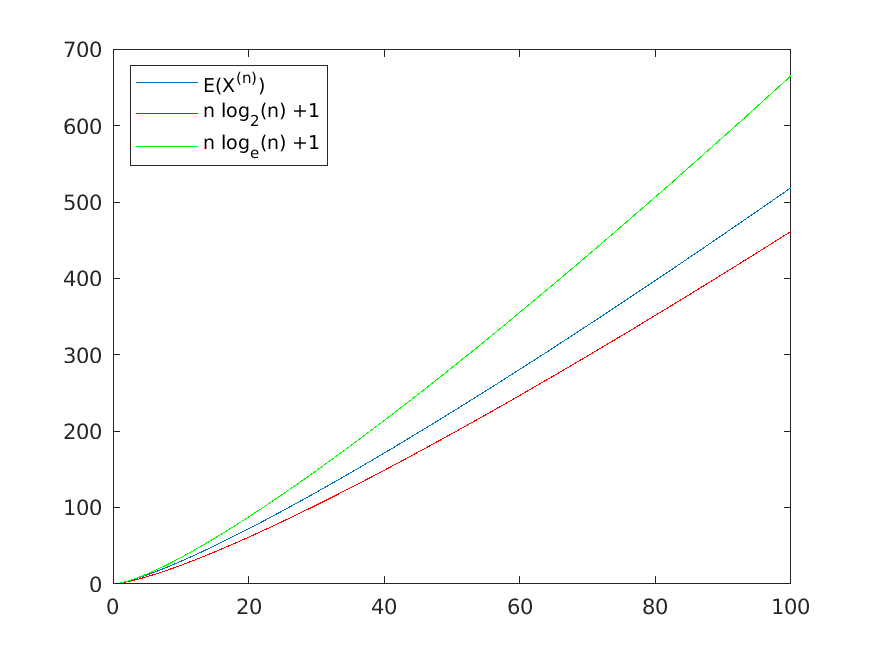
\includegraphics[width=0.8\linewidth]{q1.png}
    \caption{Plot of $E(X^{(n)})$ versus $n$ \& bounding it with $n\  log_2 (n) + 1$ \& $n\ log_e (n) + 1$}
\end{figure}
\vspace{3em}
$$\boxed{E(X^{(n)}) = \Theta(f(n))$ where $f(n) = n\ log(n)}$$


\newpage
\section*{Question 2}
\addcontentsline{toc}{section}{Question 2}
\setcounter{equation}{0}

\subsection*{(a)}
Let $U$ be a random variable distributed as a $[0,1]$ uniform distribution, thus $\{u_i\}^{n}_{i=1}$ follows the same distribution as $U$\\
Thus,
\begin{equation}
    \label{eq:uniform}
     P(U \le u) = u 
\end{equation}

Let $V$ be a random variable such that $V = F^{-1}(U)$, thus $\{v_i\}^{n}_{i=1}$ follows the same distribution as $V$  \\
Thus PMF for $V$ is,
$$
\begin{aligned}
    P(V \le x) &= P(F^{-1}(U) \le x)\\
    &= P(U \le F(x)) \hspace{1em} \text{(Since $F$ is invertible and increasing)}\\
    &= F(x) \hspace{2em} \text{(Using (\ref{eq:uniform}))}
\end{aligned}
$$
Thus, $V$ is distributed as $F$.





\newpage
\section*{Question 3}
\addcontentsline{toc}{section}{Question 3}
\setcounter{equation}{0}
We shall try proving a much more general result for an hyperplane in $n$ dimensional space.\\
Let the equation characterizing the hyperplane $z$ be written as $a_1x_1 + a_2x_2 + \ldots + a_nx_n + b + \varepsilon $\\
Representing in vector form, $z = \mathbf{a}^T\mathbf{x} + b + \varepsilon$ where $\mathbf{a} = [a_1 \ldots a_n]^T \in \mathbb{R}^n$, $\mathbf{x} = [x_1 \ldots x_n]^T \in \mathbb{R}^n$ and $b \in \mathbb{R}$ and $\varepsilon$ is the gaussian noise.\\
Thus, as the noise $\varepsilon \thicksim \mathcal{N}(0, \sigma^2)$, 
$ z_i \thicksim \mathcal{N}( \mathbf{a}^T\mathbf{x_i}+b, \sigma^2) $ where $i$ denotes the $i^{th}$ sample point.\\
Thus the likelihood $p(\{z_i\}_i;\mathbf{x_i}, \mathbf{a}, b)$ is given as:
\begin{equation*}
    \begin{split}
        p(\{z_i\}_i;\mathbf{x_i}, \mathbf{a}, b) = \prod_{i=1}^{N}\frac{1}{\sigma\sqrt{2\pi}} \exp{\bigg(\frac{(z_i - (\mathbf{a}^T\mathbf{x_i} + b))^2}{2\sigma^2}\bigg)}
    \end{split}
\end{equation*}
Taking the $\log$, we obtain the log likelihood:
\begin{equation}
    \label{logl}
    \begin{split}
        \boxed{\mathcal{L} = \log{p(\{z_i\}_i;\mathbf{x_i}, \mathbf{a}, b)} = -\frac{1}{{2\sigma^2}}\sum_{i=1}^{N} (z_i - (\mathbf{a}^T\mathbf{x_i} + b))^2 - N\log(\sigma\sqrt{2\pi})}
    \end{split}
\end{equation}
Next, we compute the partial derivatives of $\mathcal{L}$ w.r.t the parameters and equate them to 0.
\begin{equation*}
    \begin{split}
        \frac{\partial \mathcal{L}}{\partial \mathbf{a}} = \bigg( \frac{\partial \mathcal{L}}{\partial a_1}, \ldots, \frac{\partial \mathcal{L}}{\partial a_n} \bigg) = \mathbf{0} = (0, \dots, 0) \text{ and } \frac{\partial \mathcal{L}}{\partial b} = 0 
    \end{split}
\end{equation*}
Thus,
\begin{equation*}
    \begin{split}
        \frac{\partial \mathcal{L}}{\partial \mathbf{a}} = \mathbf{0} \Rightarrow \frac{\partial \mathcal{L}}{\partial a_j} = 0 \ \forall \ j = 1,\ldots,n
    \end{split}
\end{equation*}
Note that $i = 1,\ldots,N$ and $j = 1,\ldots,n$\\
\begin{equation*}
    \begin{split}
        \frac{\partial \mathcal{L}}{\partial a_j} = \frac{1}{{\sigma^2}}\sum_{i=1}^{N} (z_i - (\mathbf{a}^T\mathbf{x_i} + b))\frac{\partial (\mathbf{a}^T\mathbf{x_i})}{\partial a_j} = \frac{1}{{\sigma^2}}\sum_{i=1}^{N} (z_i - (\mathbf{a}^T\mathbf{x_i} + b))x_{ij} = 0
    \end{split}
\end{equation*}
and,
\begin{equation*}
    \begin{split}
        \frac{\partial \mathcal{L}}{\partial b} = \frac{1}{{\sigma^2}}\sum_{i=1}^{N} (z_i - (\mathbf{a}^T\mathbf{x_i} + b)) = 0
    \end{split}
\end{equation*}
Thus, we get:
\begin{equation}
    \label{set1}
    \begin{split}
        \boxed{\sum_{i=1}^{N} x_{ij}(\mathbf{a}^T\mathbf{x_i}) + b\sum_{i=1}^{N}(x_{ij}) = \sum_{i=1}^{N} (z_ix_{ij}) \  \ \forall \ j = 1,\ldots,n}
    \end{split}
\end{equation}
and,
\begin{equation}
    \label{set2}
    \begin{split}
        \boxed{\sum_{i=1}^{N}\big((\mathbf{a}^T\mathbf{x_i}) + b\cdot1 \big) = \sum_{i=1}^{N} z_i}
    \end{split}
\end{equation}
Thus we have $n+1$ equations for $n+1$ variables.

We can condense \eqref{set1} and \eqref{set2} into a single equation in the form of matrices and vectors as:
\begin{equation}
    \sum_{i=1}^{N}
    \begin{bmatrix}
        z_i x_{i1} \\
        z_i x_{i2} \\
        \vdots \\
        z_i x_{in} \\
        z_i \\
    \end{bmatrix}
    =
    \sum_{i=1}^{N}
    \begin{bmatrix}
        x_i \\
        x_2 \\
        \vdots \\
        x_n \\
        1 \\
    \end{bmatrix}
    \begin{bmatrix}
        x_i & x_2 & \cdots & x_n & 1 \\
    \end{bmatrix}
    \begin{bmatrix}
        a_i \\
        a_2 \\
        \vdots \\
        a_n \\
        b \\
    \end{bmatrix}
\end{equation}

\subsection*{(a)}
Given $z = ax + by +c$. \\
As the noise $\varepsilon \thicksim \mathcal{N}(0, \sigma^2)$, we have $ z_i \thicksim \mathcal{N}(a x_i + b y_i + c, \sigma^2) $ where $i \in (0, N)$ denotes the $i^{th}$ sample point. \\
Thus the likelihood $p(\{z_i\}_i; \{x_i\}, a, b, c)$ is given as:
\begin{equation*}
    \begin{split}
        p(\{z_i\}; \{x_i\}, \{y_i\}, a, b, c) = \prod_{i=1}^{N}\frac{1}{\sigma\sqrt{2\pi}} \exp{\bigg(\frac{(z_i - (ax_i + by_i + c))^2}{2\sigma^2}\bigg)}
    \end{split}
\end{equation*}
Taking the $\log$, we obtain the log likelihood:
\begin{equation}
    \label{logl1}
    \begin{split}
        \boxed{\mathcal{L} = \log{p(\{z_i\}; \{x_i\}, \{y_i\}, a, b, c)} = - n\log(\sigma\sqrt{2\pi}) -\frac{1}{{2\sigma^2}}\sum_{i=1}^{N} (z_i - (ax_i + by_i + c))^2 }
    \end{split}
\end{equation}
Next, we compute the partial derivatives of $\mathcal{L}$ w.r.t the parameters (a, b, c) and equate them to 0.
\begin{equation*}
    \begin{split}
        \frac{\partial \mathcal{L}}{\partial a} &= \frac{1}{{\sigma^2}}\sum_{i=1}^{N} (z_i - (ax_i + by_i + c)) x_i = 0 \Longrightarrow \sum_{i=1}^{N} z_ix_i = \sum_{i=1}^{N} (ax_i + by_i + c)) x_i \\
        \frac{\partial \mathcal{L}}{\partial b} &= \frac{1}{{\sigma^2}}\sum_{i=1}^{N} (z_i - (ax_i + by_i + c)) y_i = 0 \Longrightarrow \sum_{i=1}^{N} z_iy_i = \sum_{i=1}^{N} (ax_i + by_i + c)) y_i \\
        \frac{\partial \mathcal{L}}{\partial c} &= \frac{1}{{\sigma^2}}\sum_{i=1}^{N} (z_i - (ax_i + by_i + c)) = 0 \Longrightarrow \sum_{i=1}^{N} z_i = \sum_{i=1}^{N} (ax_i + by_i + c)) \\
    \end{split}
\end{equation*}
Matrix form:
\begin{equation}
    \sum_{i=1}^{N}
    \begin{bmatrix}
        z_i x_i \\
        z_i y_i \\
        z_i \\
    \end{bmatrix}
    =
    \sum_{i=1}^{N}
    \begin{bmatrix}
        x_i^2 & x_i y_i & x_i \\
        x_i y_i & y_i^2 & y_i \\
        x_i & y_i & 1 \\
    \end{bmatrix}
    \begin{bmatrix}
        a \\
        b \\
        c \\
    \end{bmatrix}
    =
    \sum_{i=1}^{N}
    \begin{bmatrix}
        x_i \\
        y_i \\
        1 \\
    \end{bmatrix}
    \begin{bmatrix}
        x_i & y_i & 1 \\
    \end{bmatrix}
    \begin{bmatrix}
        a \\
        b \\
        c \\
    \end{bmatrix}
\end{equation}

\subsection*{(b)}
Given $z = f(x,y) = a_1 x^2 + a_2 y^2 + a_3 xy + a_4 x + a_5 y + a_6$. \\
As the noise $\varepsilon \thicksim \mathcal{N}(0, \sigma^2)$, we have $ z_i \thicksim \mathcal{N}(f(x_i, y_i), \sigma^2) $ where $i \in (0, N)$ denotes the $i^{th}$ sample point. \\
Thus the likelihood $p(\{z_i\}_i; \{x_i\}, a_1, a_2, a_3, a_4, a_5, a_6)$ is given as:
\begin{equation*}
    \begin{split}
        p(\{z_i\}; \{x_i\}, \{y_i\}, a_1, a_2, a_3, a_4, a_5, a_6c) = \prod_{i=1}^{N}\frac{1}{\sigma\sqrt{2\pi}} \exp{\bigg(\frac{(z_i - (f(x_i,y_i))^2}{2\sigma^2}\bigg)}
    \end{split}
\end{equation*}
Taking the $\log$, we obtain the log likelihood:
\begin{equation}
    \label{logl1}
    \begin{split}
        \boxed{\mathcal{L} = \log{p(\{z_i\}; \{x_i\}, \{y_i\}, a_1, a_2, a_3, a_4, a_5, a_6)} = - n\log(\sigma\sqrt{2\pi}) -\frac{1}{{2\sigma^2}}\sum_{i=1}^{N} (z_i - (f(x_i,y_i))^2 }
    \end{split}
\end{equation}
Next, we compute the partial derivatives of $\mathcal{L}$ w.r.t the parameters and equate them to 0.
\begin{equation*}
    \begin{split}
        \frac{\partial \mathcal{L}}{\partial a_1} &= \frac{1}{{\sigma^2}}\sum_{i=1}^{N} (z_i - f(x_i,y_i)) x_i^2 = 0 \Longrightarrow \sum_{i=1}^{N} z_i x_i^2 = \sum_{i=1}^{N} (a_1 x_i^2 + a_2 y_i^2 + a_3 x_iy_i + a_4 x_i + a_5 y_i + a_6) x_i^2\\
        \frac{\partial \mathcal{L}}{\partial a_2} &= \frac{1}{{\sigma^2}}\sum_{i=1}^{N} (z_i - f(x_i,y_i)) y_i^2 = 0 \Longrightarrow \sum_{i=1}^{N} z_i y_i^2= \sum_{i=1}^{N} (a_1 x_i^2 + a_2 y_i^2 + a_3 x_iy_i + a_4 x_i + a_5 y_i + a_6) y_i^2\\
        \frac{\partial \mathcal{L}}{\partial a_3} &= \frac{1}{{\sigma^2}}\sum_{i=1}^{N} (z_i - f(x_i,y_i)) x_iy_i = 0 \Longrightarrow \sum_{i=1}^{N} z_i x_iy_i= \sum_{i=1}^{N} (a_1 x_i^2 + a_2 y_i^2 + a_3 x_iy_i + a_4 x_i + a_5 y_i + a_6) x_iy_i\\
        \frac{\partial \mathcal{L}}{\partial a_4} &= \frac{1}{{\sigma^2}}\sum_{i=1}^{N} (z_i - f(x_i,y_i)) x_i = 0 \Longrightarrow \sum_{i=1}^{N} z_i x_i= \sum_{i=1}^{N} (a_1 x_i^2 + a_2 y_i^2 + a_3 x_iy_i + a_4 x_i + a_5 y_i + a_6) x_i\\
        \frac{\partial \mathcal{L}}{\partial a_5} &= \frac{1}{{\sigma^2}}\sum_{i=1}^{N} (z_i - f(x_i,y_i)) y_i = 0 \Longrightarrow \sum_{i=1}^{N} z_i y_i= \sum_{i=1}^{N} (a_1 x_i^2 + a_2 y_i^2 + a_3 x_iy_i + a_4 x_i + a_5 y_i + a_6) y_i\\
        \frac{\partial \mathcal{L}}{\partial a_6} &= \frac{1}{{\sigma^2}}\sum_{i=1}^{N} (z_i - f(x_i,y_i)) = 0 \Longrightarrow \sum_{i=1}^{N} z_i = \sum_{i=1}^{N} (a_1 x_i^2 + a_2 y_i^2 + a_3 x_iy_i + a_4 x_i + a_5 y_i + a_6)\\
    \end{split}
\end{equation*}
Matrix form:
\begin{equation}
    \sum_{i=1}^{N}
    \begin{bmatrix}
        z_i x_i^2 \\
        z_i y_i^2 \\
        z_i x_i y_i \\
        z_i x_i \\
        z_i y_i \\
        z_i \\
    \end{bmatrix}
    =
    \sum_{i=1}^{N}
    \begin{bmatrix}
        x_i^2 \\
        y_i^2 \\
        x_i y_i \\
        x_i \\
        y_i \\
        1 \\
    \end{bmatrix}
    \begin{bmatrix}
        x_i^2 & y_i^2 & x_i y_i & x_i & y_i & 1 \\
    \end{bmatrix}
    \begin{bmatrix}
        a_1 \\
        a_2 \\
        a_3 \\
        a_4 \\
        a_5 \\
        a_6 \\
    \end{bmatrix}
\end{equation}

\subsection*{(c)}
\subsection*{Instructions for running the code:}
\begin{itemize}
    \item After extracting submitted file, look for a directory named \texttt{code}.
    \item Within this, the code for this question is contained in a directory named \texttt{q3}
    \item Run the file \texttt{q3.m} for predicting the equation of the plane and noise variance.
\end{itemize}
On running the code with \texttt{XYZ.txt} as the input file, \\
Output:
\begin{figure}[H]
    \vspace{-1em}
    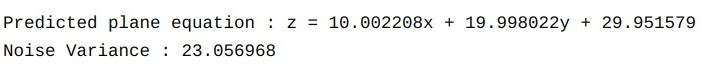
\includegraphics[width=0.8\linewidth, left]{output.jpeg}
\end{figure}
\vspace{-1em}
Thus, the predicted equation of plane is \boxed{$z = 10x + 20y + 30$} and noise variance is \boxed{23}.


\newpage
\section*{Question 4}
\addcontentsline{toc}{section}{Question 4}
\setcounter{equation}{0}
There are $N\ (=1000)$ samples in our dataset ($X$).\\
There are $n\ (=750)$ samples in our training set.\\
There are $m\ (=250)$ samples in our validation set.\\
Let the training set $T$ be given by $T = \{t_i\}_{i=1}^n$\\
Let the validation set $V$ be given by $V = \{v_j\}_{j=1}^m$\\
Also, $T\cap V = \phi$ and $T \cup V = X$\\
Thus, we have the Gaussian kernel estimator as:\\
$$
\hat p_n(x;\sigma) = \frac{1}{n\sigma\sqrt{2\pi}} \sum_{i=1}^{n}\exp\bigg(\frac{-(x - t_i)^2}{2\sigma^2} \bigg)
$$
\subsection*{(b)}
Therefore, the joint likelihood of the samples in $V$, assuming $\{v_j\}_{j=1}^{m}$ to be independent, is:
$$
\begin{aligned}
    f(\{v_j\}_{j=1}^{m}; \sigma) &= \prod_{j=1}^m \hat p_n(v_j;\sigma)\\
    &= \Aboxed{\bigg(\frac{1}{n\sigma\sqrt{2\pi}}\bigg)^m\cdot \prod_{j=1}^m\Bigg( \sum_{i=1}^{n}\exp\bigg(\frac{-(v_j - t_i)^2}{2\sigma^2} \bigg) \Bigg)}
\end{aligned}
$$
The log-likelihood is given by:
$$
\begin{aligned}
    \log f(\{v_j\}_{j=1}^{m}; \sigma) &= \sum_{j=1}^m \log (\hat p_n(v_j;\sigma))\\
    &= \Aboxed{\sum_{j=1}^m \log \bigg(\sum_{i=1}^{n}\exp\bigg(\frac{-(v_j - t_i)^2}{2\sigma^2} \bigg)\bigg) - m\log(n\sigma\sqrt{2\pi})}
\end{aligned}
$$
\subsection*{(c)}
\begin{figure}[H]
    \centering
    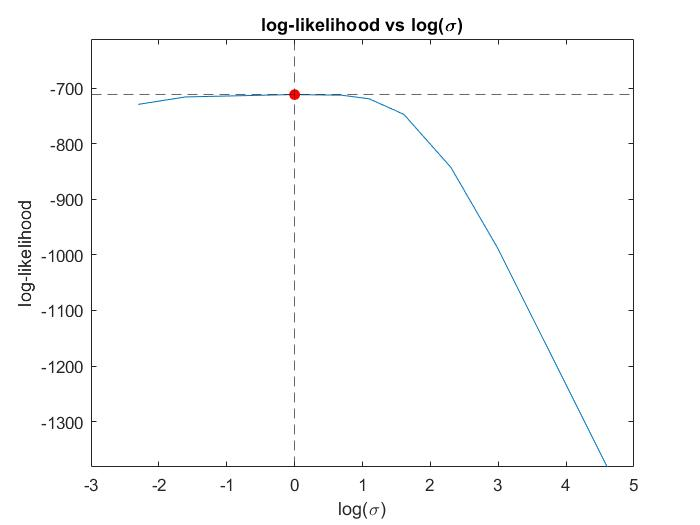
\includegraphics[scale=0.4]{q4ci.jpg}
    \caption{$\log f(\{v_j\}_{j=1}^{m}; \sigma)$ vs $\log(\sigma)$}
    \label{fig:my_label}
\end{figure}

$\boxed{\sigma = 1 }$ yields the maximum value of the log-likelihood.

\begin{figure}[H]
    \centering
    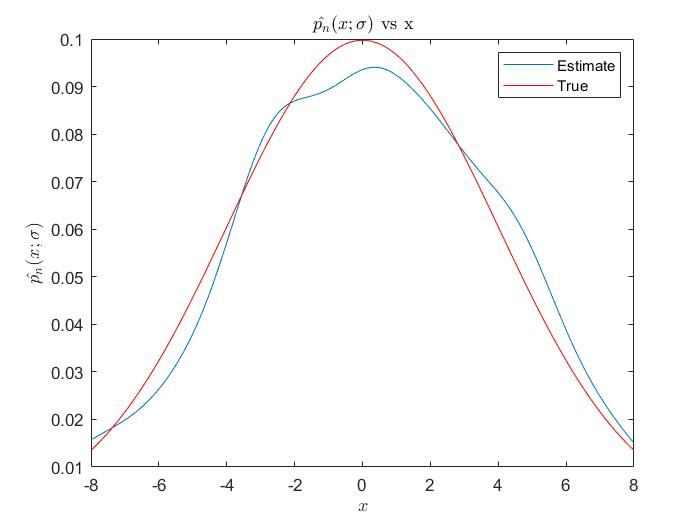
\includegraphics[scale=0.4]{q4cii.jpg}
    \caption{True PDF overlaid on the estimated PDF}
    \label{fig:my_label}
\end{figure}
\newpage

\subsection*{(d)}
\begin{figure}[H]
    \centering
    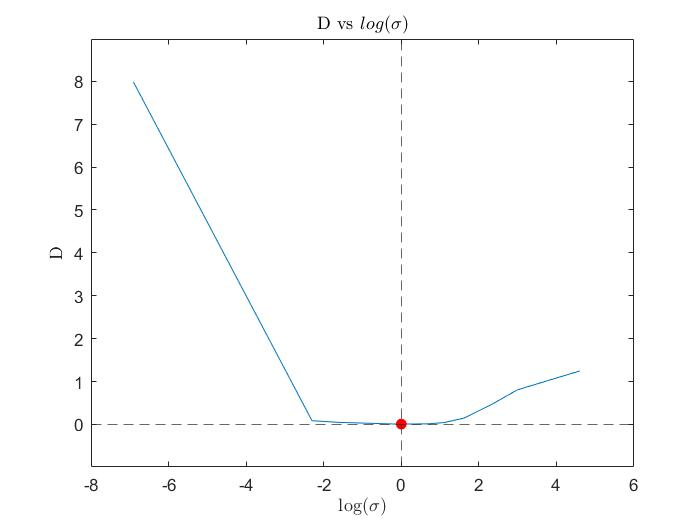
\includegraphics[scale=0.41]{q4di.jpg}
    \caption{D vs $\log(\sigma)$}
    \label{fig:my_label}
\end{figure}

\begin{figure}[H]
    \centering
    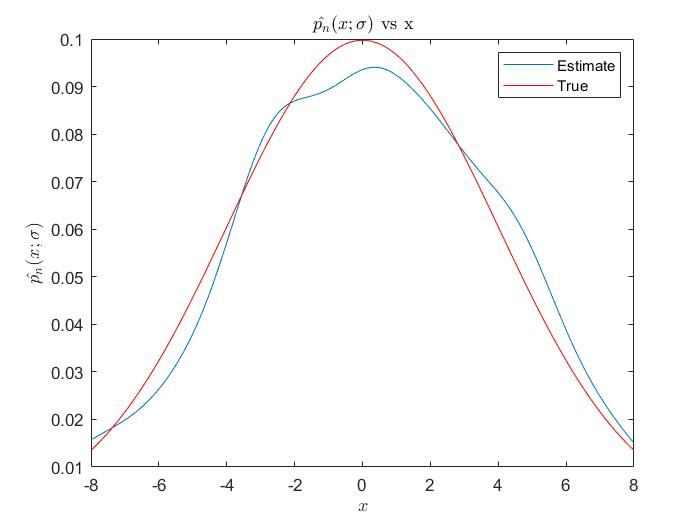
\includegraphics[scale=0.41]{q4cii.jpg}
    \caption{True PDF overlaid on the estimated PDF}
    \label{fig:my_label}
\end{figure}
\newpage

\begin{verbatim}
    Best sigma that minimizes D:  0.9000
    The value of D at this sigma(= 0.9000) is:  0.0048
    D value for the sigma parameter that yielded the best LL:  0.0049
\end{verbatim}

\subsection*{(e)}

\end{document}
